\documentclass[preprint,showpacs,amssymb,amsmath,aps,prb]{revtex4}
\setcitestyle{numbers,square}
\usepackage{graphics}
\usepackage{graphicx}
%\usepackage{hyperref}
\usepackage{bm}
\usepackage{bbm}
\usepackage{amsmath}
\usepackage{amssymb}
%\usepackage{underscore}
%\usepackage{bbm}
\usepackage{dsfont}
\begin{document}

\title{Pair entanglement in dimerized spin-$s$ chains}
\author{A.\ Boette, R.\ Rossignoli, N.\ Canosa, J.\ M.\ Matera}
\affiliation{Departamento de F\'isica-IFLP, 
Universidad Nacional de La Plata, C.C. 67, La Plata (1900), Argentina}
\begin{abstract}
We examine the pair entanglement in the ground state of
finite dimerized spin $s$ chains interacting through anisotropic $XY$ couplings
immersed in a transverse magnetic field, by means of a self-consistent pair
mean field approximation. The approach, which makes no a priori assumptions on
the pair states, predicts, for sufficiently low coupling between pairs, $2s$
distinct dimerized phases for increasing fields below the pair factorizing
field, separated by spin parity breaking phases. The dimerized phases lead to
approximate magnetization and pair entanglement plateaus, while the parity
breaking phases are characterized by weak pair entanglement but non-negligible
entanglement of the pair with the rest of the system. These predictions are
confirmed by the exact results obtained in finite $s=1$ and $s=3/2$ chains. It
is also shown that for increasing values of the spin $s$, the entanglement of
an isolated pair, as measured by the negativity, rapidly saturates in the
anisotropic $XY$ case  but increases as $s^{1/2}$ in the $XX$ case, reflecting
a distinct single spin entanglement spectrum.

\end{abstract} \pacs{03.65.Ud,03.67.Mn,75.10.Jm,64.70.Tg}

\maketitle
\section{Introduction}

%\bibitem{SR.09} S.\ Rachel, .
%\bibitem{MV.12}F.\ Michaud, et al y M.  Lajko et al.
%\bibitem{KM.08}V.\ Karimipour et al

The study of entanglement in interacting spin systems has received strong
attention in recent years \cite{Am.08,ECP.10}. Entanglement has provided a
novel perspective for the  analysis of correlations and quantum phase
transitions \cite{Am.08,ECP.10,ON.02}, being also essential for
determining the potential  of such systems in the field of quantum information
\cite{NC.00}. Interest in spin systems has  been enhanced  by the impressive
advances in  control techniques of quantum systems \cite{HR.06},  that have
made it possible to  simulate interacting spin models with different type of
couplings by means of  trapped ions, Josephson junctions and cold atoms in
optical lattices \cite{PC.04,GA.14,BR.12,SR.15,B.16,LS.12}.

In particular, dimerized systems, characterized by strongly coupled spin pairs
$\bf{and}$ arising from various possible geometric configurations and  couplings
\cite{Pr.75,Pr.77,FM.07,GG.09,CRM.10,MG.69,S.05,KSV.07,HXG.08,HH.11,Mn.14,LM.15,BRCM.15,ORSB.15},
are of great interest, providing a basis for understanding magnetization
plateaus and non-trivial magnetic behavior \cite{ORSB.15}. They have also been
recently simulated with cold atoms in optical lattices \cite{ZZ.14}. 
While the basic case deals with singlet pairs
in antiferromagnetic (AFM)-like systems \cite{LM.15}, other types of
dimerization can also arise in the ground state (GS) of systems with
non-uniform couplings, like spin chains with alternating-type $XYZ$
couplings \cite{Pr.75,Pr.77,FM.07,GG.09,CRM.10,HXG.08,BRCM.15,LM.15}. In
these systems a basic mean field approximation (MF) based on independent spins
clearly fails to provide even the most basic features of the GS and its
magnetic behavior. Instead, we have shown \cite{BRCM.15}  that a pair MF
approach, a particular case of a generalized cluster-type variational mean
field treatment, based on independent pairs whose state is self-consistently
determined and admitting relevant symmetry-breaking, is able to provide a
correct basic description. In dimerized spin $1/2$  arrays with
anisotropic $XY$ and $XYZ$ couplings the approach is in fact analytic,
providing a phase diagram that differs from that of the standard  MF and
contains a (single) dimerized phase at low fields under appropriate conditions
\cite{BRCM.15}. Such prediction is in good agreement with the exact results,
which in the special case of spin $1/2$ chains with first neighbor $XY$
couplings can  be analytically obtained through the Jordan-Wigner 
fermionization \cite{LSM.61,Pr.75,Pr.77,CRM.10}.

The aim of this work is to extend previous results to spin $s$ systems with
$s\geq 1$, where the previous fermionization is no longer available and
where the system Hilbert space dimension becomes rapidly very large  for exact
numerical solutions as the total number of spins increases. In this scenario we
will show that the self-consistent pair MF approach constitutes a convenient method
for understanding the basic physics,  which can still depart considerably from
the conventional MF prediction and the bosonic-like behavior expected for high
spin \cite{MRC.10}. The approach also provides an accurate description of the
reduced state of pairs, enabling to determine   the main  features of the
pair entanglement. In particular, for sufficiently low coupling and appropriate
anisotropies, the approach predicts  $2s$  dimerized phases for increasing
fields below the factorizing field \cite{KTM.82}, characterized by
magnetization and pair entanglement approximate plateaus, which are separated
by $S_z$ parity breaking phases where the pair entanglement drops considerably
while that of the pair with the remaining chain becomes non-negligible. These
features are confirmed by the exact numerical results obtained in small finite
spin $1$ and $3/2$ chains. We will also analyze the behavior for large spin,
showing the distinct entanglement properties of anisotropic $XY$ and $XX$
pairs. The formalism and its application to  dimerized spin $s$ $XY$ systems is
described  in sec.\ \ref{II}, while results are discussed in detail in sec.\
\ref{III}.  Conclusions are given in \ref{IV}.

\section{Formalism \label{II}}

\subsection{Pair mean field in dimerized arrays and parity breaking}

We consider a finite chain of $2n$ spins $s$ in a transverse uniform field $B$
interacting through alternating first neighbor anisotropic $XY$ couplings 
\cite{Pr.75,Pr.77,FM.07,GG.09,CRM.10}, such that the chain contains strongly
coupled pairs weakly interacting with their neighboring pairs. The Hamiltonian
can be written as 
\begin{equation}
H=\sum_{i=1}^n [B (S^z_{2i-1}+S^z_{2i})-\sum_{\mu=x,y}J_\mu(S_{2i-1}^\mu
 S_{2i}^\mu+\alpha S_{2i}^\mu S_{2i+1}^\mu)]\,, \label{H1}\end{equation}
where $S_i^\mu$ are the spin components at site $i$ (with
$S_{2n+1}^\mu=S_{1}^\mu$ ($0$) in the cyclic (open) case),  $J_\mu$ are the
exchange couplings and the parameter $\alpha$ indicates the relative strength
of the coupling between pairs ($|\alpha|\leq 1$).  Without loss of generality
we can assume (for even $n$ in the cyclic case) $\alpha\geq 0$ and $J_x\geq 0$,
as their signs can be changed by local rotations around the $z$ axis. We can
obviously also set $B\geq 0$ (its sign is changed by a global rotation around
the $y$ axis) and $|J_y|\leq J_x$. The relevant symmetry for $J_y\neq J_x$ is
the $S^z$ parity  $P_z=\exp[\imath
2\pi\sum_{i=1}^{2n}(S_{i}^z+s)]=\prod_{i=1}^{2n} P_{zi}$, which satisfies
$[P_z,H]=0$.

In a  pair mean field (MF) treatment, the GS of (\ref{H1}) is approximated by a
pair product state $|\Psi_{0}\rangle=\prod_{i=1}^n|\psi_{0i}\rangle$, with
$|\psi_{0i}\rangle$ the state of  the pair $(2i-1,2i)$.  Minimization of
$E_0=\langle \Psi_0|H|\Psi_0\rangle$ then leads to the independent pair
self-consistent Hamiltonian $h=\sum_{i=1}^n h_i$, with
\begin{equation}
h_i=B (S^z_{2i-1}+S^z_{2i})-\sum_{\mu}J_\mu [S_{2i-1}^\mu
 S_{2i}^\mu+\alpha(S_{2i}^\mu \langle S_{2i+1}^\mu\rangle+
 \langle S_{2i-2}^\mu\rangle S_{2i-1}^\mu)]\,, \label{h}\end{equation}
 where
$\langle S^\mu_{2i+j}\rangle=\langle\psi_{0i}|S^\mu_{2i+j}|\psi_{0i}\rangle$,
$i=1,\ldots,n$, $j=-1,0$, are the mean values in the GS $|\psi_{0i}\rangle$ of
$h_i$ ({\it self-consistency conditions}).  The internal coupling of the pair
is treated {\it exactly}. The energy is then $E_0=\sum_{i=1}^n[\langle
h_i\rangle+\alpha\sum_\mu J_\mu \langle S_{2i}\rangle\langle S_{2i+1}\rangle]$.

In the ferromagnetic (FM) setting considered, we may assume in the cyclic case a
uniform pair mean field such that  $\langle S^\mu_{2i-1}\rangle=\langle
S^\mu_{2i}\rangle\equiv\langle S^\mu\rangle$ independent of $i$ (unbroken
translational symmetry), with $\langle S^y\rangle=0$ for the lowest energy mean
field if $|J_y|<J_x$.  Hence, the pair mean field will be characterized by a
single parity breaking order parameter $\langle S^x\rangle$: If $\langle
S^x\rangle=0$ it leads to a parity preserving {\it dimerized phase} at the pair
MF level, with no average coupling  between pairs, while if $\langle
S^x\rangle\neq 0$ it corresponds to  a {\it parity breaking phase}, with
non-zero coupling  between pairs. This last phase is, of course, twofold
degenerate for $|J_y|<J_x$, as both signs $\langle S^x\rangle=\pm|\langle
S^x\rangle|$ are equally possible, with
$|\psi_{0i}^-\rangle=P_{zi}|\psi_{0i}^+\rangle$. At the parity breaking phases
we will then consider the definite parity combinations
\begin{equation}|\Psi_{0\pm}\rangle\propto(\mathds{1}\pm P_z)\prod_{i=1}^n|\psi_{0i}^+\rangle
=\prod_{i=1}^n|\psi_{0i}^+\rangle+\prod_{i=1}^n|\psi_{0i}^-\rangle\label{pmfr}\,,
\end{equation}
satisfying $P_z|\Psi_{0\pm}\rangle=\pm|\Psi_{0\pm}\rangle$, selecting that of
lower energy. These states lead to a finite entanglement between pairs.

In order to determine the onset of parity-breaking, we may consider the first
order expansion of the common pair ground state
$|\psi_0\rangle=|\psi_{0i}\rangle$ for small $\langle S^x \rangle$,
 $|\psi_0\rangle \approx |\psi_0^0\rangle + |\delta \psi_0\rangle$,
where $|\delta \psi_0\rangle =\alpha J_x\langle S^x\rangle \sum_{k>0}
\frac{\langle \psi_k^0| S^x_t|\psi_0^0\rangle}{E_k-E_0}|\psi_k^0\rangle$, with
$S^x_t=S^x_{1}+S^x_{2}$ and  $\{|\psi_k^0\rangle\}$ the eigenstates of the
$\langle S^x\rangle=0$ pair Hamiltonian $h^0$:
$h^0|\psi^0_k\rangle=E_k|\psi^0_k\rangle$. Since pair parity symmetry, exactly
conserved in $h^0$, implies $\langle\psi_0^0|S^x_t|\psi_0^0\rangle=0$
(assuming $|\psi_0^0\rangle$ non-degenerate) we have $\langle S^x\rangle\approx 
{\rm Re}[\langle \psi_0^0|S^x_t|\delta\psi_0\rangle]$ up to first order in 
$\langle S^x\rangle$, implying the critical condition
\begin{equation}
1=\alpha J_x\sum_{k>0}\frac{|\langle\psi_k^0|S^x_t|\psi_0^0\rangle|^2}{E_k-E_0}
\,. \label{crit}\end{equation}
 Parity breaking is then feasible if
\begin{equation}\alpha>\frac{1}{J_x \sum_{k>0}
\frac{|\langle \psi_k^0|S^x_t|\psi_0^0\rangle|^2}{E_k-E_0}}
\,.\label{alphac}\end{equation}
Eq.\ (\ref{crit}) determines a {\it finite} threshold value for $\alpha$
whenever the isolated pair is {\it gapped} ($E_k-E_0>0$ $\forall$ $k>0$), which
will depend on the relative field strength $B/J_x$, the ratio $\chi=J_y/J_x$
and the spin $s$. The sum in (\ref{crit}) is typically exhausted by the first
term $\frac{|\langle \psi_1^0|S^x_t|\psi_0^0\rangle|^2}{E_1-E_0}$ with $E_1$ 
the lowest energy of $S^z$ parity opposite to that of $E_0$. 
 We also have the  restriction $\alpha\leq 1$, which sets
an upper bound on $B/J_x$ ($B<B_{c}^p$).

On the other hand, the threshold value {\it vanishes} when the smallest
excitation energy  $E_1-E_0$ becomes zero. Hence, pair GS level crossings will
separate  distinct dimerized phases at sufficiently low $\alpha$, leading to
several onsets (and ``deaths'') of parity breaking as the field increases, as
shown in the next section. For $s=1/2$   there are \cite{BRCM.15} two parity
preserving  phases if $\chi>0$ and  $\alpha<\frac{1}{2}\chi$, with parity
breaking in  a {\it single} field window $B_{c1}<B<B_{c2}$.

Such multiple dimerized phases are obviously absent in the conventional single
spin MF (full product state approximation), which in this system becomes
equivalent to the  MF treatment of a standard chain with uniform coupling of
strength $J_x(1+\alpha)/2$, being independent of $J_y$ if $|J_y|<J_x$. For any
spin $s$ it leads to a single parity breaking phase for $|B|<B_{c}^{\rm
mf}\equiv J_xs(1+\alpha)$, where $\langle S_x\rangle=\pm s\sin\theta$ with
$\cos\theta=B/B_c^{\rm mf}$.

Nevertheless, for $0<J_y<J_x$ there is one point where {\it both} the single
spin and pair mean field treatments coincide and become rigorously {\it exact}
for {\it any} value of the spin $s$  and the number $n$ of spins, i.e., where
the chain GS completely forgets its dimerized structure, which is the {\it
factorizing field} \cite{CRM.10,BRCM.15}
 \begin{equation}B_s=J_xs(1+\alpha)\sqrt{\chi}\,,
 \;\;\;\chi=J_y/J_x\,.\label{Bs}\end{equation}
At this field the chain exhibits a pair of degenerate {\it completely
separable} parity breaking aligned ground states
\begin{equation}|\pm\Theta\rangle=|\pm\theta,\pm\theta,\ldots\rangle\,,
\label{ths}\end{equation}
with $|\pm\theta\rangle=e^{\mp i\theta S^y}|-s\rangle$ a single spin state with
maximum spin forming an angle $\pm\theta$ with the $-z$ axis, with
$\cos\theta=B_s/B_c^{\rm mf}=\sqrt{\chi}$. In a finite chain the factorizing
field (\ref{Bs}) is actually that where the {\it last} GS parity transition
takes place\cite{RCM.08,RCM.09} (see next section). Accordingly, the
side-limits of the exact GS at $B_s$ in a finite chain will not be given by the
product states (\ref{ths}) but rather by the definite parity combinations
$|\Theta_{\pm}\rangle\propto |\Theta\rangle\pm|-\Theta\rangle$, with
$P_z|\Theta_{\pm}\rangle=\pm|\Theta_{\pm}\rangle$ \cite{RCM.08,RCM.09}, which
will then be correctly predicted by the symmetry-restored pair MF states
(\ref{pmfr}). A GS transition $|\Theta_-\rangle\rightarrow|\Theta_+\rangle$
will then take place as $B$ crosses $B_s$.

For AFM type couplings ($J_x<0$ and/or $\alpha<0$ in (\ref{H1})), factorizing
and critical values of $B$ and $\alpha$  take exactly the same previous values.
Just suitable local rotations are to be applied to the corresponding state. For
instance, if $J_x>0$ but $\alpha<0$, they will transform the previous uniform
pair state into a Neel type pair state
$|\Psi_0\rangle=|\psi_{0}\rangle|\tilde{\psi}_{0}\rangle|\psi_0\rangle\ldots$
with $|\tilde{\psi}_0\rangle=e^{-i\pi(S_1^z+S_2^z)}|\psi_0\rangle\propto
P_{z}|\psi_0\rangle$ and $\langle S^x\rangle_{2i+j}=(-1)^{i-1} \langle
S^x\rangle$ for $j=0,-1$. These rotations will not affect the energy spectrum
nor entanglement measures.

The pair MF approach can of course be applied to more complex couplings and geometries. 
For instance, if the coupling between pairs $i$ and $i+1$ contains  
 second and third neighbor terms, such that it is of the form 
$-\sum_{\mu}J_\mu\sum_{j,l=1,2}\alpha_{jl}S_{2i-2+j}^\mu S_{2i+l}^\mu$ 
we should just replace the $\alpha$-term in (\ref{h}) by $\sum_{j,l=1,2}S^\mu_{2i-2+j}(\alpha_{jl}\langle S^\mu_{2i+l}\rangle+\alpha_{lj}
\langle S^{\mu}_{2i-4+l}\rangle)$. If translational symmetry remains unbroken, 
as will occur for $\alpha_{jl}\geq 0$ $\forall$ $j,l$,  previous equations can be directly applied, leading to the same critical condition (\ref{crit}) with $\alpha=\sum_{j,l=1,2}\alpha_{j,l}$. For different signs, the possibility of non-uniform solutions should also be considered.

 \subsection{Entanglement}
The reduced state of a strongly coupled  pair in the exact GS $|\Psi_0\rangle$
of the chain is given by $\rho_{12}={\rm
Tr}_{3,4,\ldots}|\Psi_0\rangle\langle\Psi_0|$. The entanglement of the pair
with the rest of the chain can be measured through the entanglement entropy
$S(\rho_{12})=-{\rm Tr}\rho_{12}\log_2\rho_{12}$, satisfying  $S(\rho_{12})\leq
2\log_2(2s+1)$ for a pair of spins $s$.  On the other hand, its internal
entanglement can be estimated through the negativity (an entanglement monotone
computable for mixed states of any dimension  \cite{VW.02,ZHSL.99})
\begin{equation} N_{12}=({\rm Tr}\,|\rho_{12}^{\rm t_2}|-1)/2\label{N12}\,,\end{equation}
where $\rho^{\rm t_2}$ denotes the partial transpose of $\rho_{12}$. Eq.\ (\ref{N12})
is just minus the sum of the negative eigenvalues of $\rho_{12}^{\rm t_2}$. If
 $\rho_{12}$ is pure ($\rho_{12}=|\psi_0\rangle\langle\psi_0|$) Eq.\ (\ref{N12})
 becomes a generalized  entanglement entropy,
\begin{equation}N_{12}=[({\rm Tr}\,\sqrt{\rho_1})^2-1]/2
 =\sum_{i<j}\lambda_i^1\lambda^1_j\label{N12p}\end{equation}
where $\rho_1={\rm Tr}_2\,|\psi_0\rangle\langle\psi_0|$ is the single spin
reduced state and $\lambda^1_i$ its eigenvalues.  Accordingly, Eq.\
(\ref{N12p}) vanishes for $\rho_1$ pure ($|\psi_0\rangle$ separable) and
reaches its maximum for a maximally mixed $\rho_1$  ($|\psi_0\rangle$ maximally
entangled), in which case $N_{12}=s$ for a pair of spins $s$.

At the pair MF level,  $\rho_{12}$ will be pure in the
parity preserving phases. However, in the parity breaking phases $\rho_{12}$ will become
{\it mixed}  if the parity restored states (\ref{pmfr}) are employed. The latter lead
 to a rank $2$ reduced state of the form
\begin{equation}\rho_{12}\approx \frac{1}{2}(|\psi_0^+\rangle\langle\psi_0^+|
+|\psi_0^-\rangle\langle\psi_0^-|)\,,
 \label{pbm}\end{equation}
if the complementary overlap $|\langle \psi_0^+|\psi_0^-\rangle|^{n-1}$
(negligible if $n$ and $\langle S^x\rangle$ are not too small) is discarded,
whose non-zero eigenvalues are just $\lambda_{\pm}=\frac{1}{2}(1\pm|\langle
\psi_{0}^-|\psi_0^+\rangle|)$. Hence, a non-zero entanglement entropy of the
pair with the rest of the chain will arise at the pair MF level within the
parity breaking phases, which will then satisfy $S(\rho_{12})\leq 1$,  with
$S(\rho_{12})\approx 1$  if the overlap $\langle\psi_{0}^-|\psi_0^+\rangle$ is
also negligible.

At the factorizing field (\ref{Bs}), Eq.\ (\ref{pbm}) becomes {\it exact} (if
$\langle -\theta,-\theta|\theta,\theta\rangle^{n-1}=(\cos^{4s}\theta)^{n-1}$ is
neglected), with $|\psi_0^{\pm}\rangle=|\pm\theta,\pm\theta\rangle$ product
states. Consequently, even with symmetry restoration the exact side-limits of
$\rho_{12}$ at $B_s$ will become {\it separable}, i.e. a convex combination of
product states \cite{W.89}, leading to $N_{12}=0$ at this point. Nonetheless,
it will remain {\it mixed}, with eigenvalues
$\lambda_{\pm}=\frac{1}{2}(1\pm\cos^{4s}\theta)$, implying a nonzero
entanglement of the pair with the rest of the chain at the side-limits
$B\rightarrow B_s^{\pm}$.

\section{Results\label{III}}
\subsection{The spin-1 case}
\subsubsection{The spin 1 pair}
We first examine in detail the case $s=1$. In order to understand the behavior
of both the pair MF and the exact solution for general $\alpha$ in (\ref{H1}),
we first discuss the isolated pair ($\alpha=0$). The lowest energy levels  of
the pair for each parity $P_z$ and for $|J_y|\leq J_x$ are
\begin{eqnarray}
E_+&=&{\textstyle-\sqrt{2B^2+\frac{J_x^2+J_y^2}{2}+\sqrt{4B^2(B^2-J_xJ_y)+\frac{(J_x^2+J_y^2)^2}{4}}}}\,,
\label{Ep}\\
 E_-&=&{\textstyle-[\frac{J_x+J_y}{2}+\sqrt{B^2 +\frac{(J_x-J_y)^2}{4}}]}\,,
\label{Em}
\end{eqnarray}
with  eigenstates
\begin{eqnarray}
|\psi_+\rangle&=&
\alpha_{-}|-1,-1\rangle+\alpha_0|0,0\rangle+\alpha_+|1,1\rangle+\alpha_{11}
{\textstyle\frac{|-1,1\rangle+|1,-1\rangle}{\sqrt{2}}}\,,
 \label{psip}\\
|\psi_-\rangle&=&{\textstyle\beta_-\frac{|-1,0\rangle+|0,-1\rangle}
{\sqrt{2}}+\beta_+\frac{|0,1\rangle+|1,0\rangle}{\sqrt{2}}
=\frac{|0,\phi\rangle+|\phi,0\rangle}{\sqrt{2}}}\,,\label{psim}
\end{eqnarray}
in the standard product basis $\{|m_1,m_2\rangle\}$ of eigenstates of $S^z_1$
and $S^z_2$, where \begin{eqnarray}
\alpha_0&=&{\textstyle\alpha_-\frac{2(|E_+|-2B)}{J_x-J_y},\;\;\alpha_+
=\alpha_-\frac{|E_+|-2B}{|E_+|+2B},\;\; \alpha_{11}=\alpha_0\frac{J_x+J_y}{\sqrt{2}|E_+|}}
\nonumber\\
\beta_+&=&{\textstyle\beta_-\frac{2(|E_-|-B)-(J_x+J_y)}{J_x-J_y}}\,.
\end{eqnarray}
Here  $|\psi_-\rangle$ is seen to be a Bell type state, with
$|\phi\rangle=\beta_-|-1\rangle+\beta_+|1\rangle$, whereas $|\psi_+\rangle$ has
full Schmidt rank if $J_y\neq J_x$. For strong fields $B\gg J_x$, $E_+\approx
-2B$, $E_-\approx -B$, while for zero field $E_+=-J_x\sqrt{1+\chi^2}$,
$E_-=-J_x$, so that $|\psi_+\rangle$ is the GS in these limits. Yet if
$\chi=J_y/J_x\in(0,1]$,  $|\psi_-\rangle$ will be the GS in an intermediate
field window $B_{c1}\leq B\leq B_{c2}$, as seen in the inset of Fig.\ \ref{f2},
with
\begin{eqnarray}
 B_{c1}&\approx &\sqrt{\chi}J_x{\textstyle\frac{(1-4\chi/25)}{\sqrt{5}}}\label{bc1},\;\;
 B_{c2}=\sqrt{\chi}J_x=B_s\,,\end{eqnarray}
where the expression for $B_{c1}$ holds for small $\chi$ and $B_s$ is the {\it
separability field} (\ref{Bs}) for the isolated pair ($\alpha=0$). Hence, for
$\chi>0$ the pair GS will undergo two parity transitions as the field increases
from 0, the last one at $B_s$.  These transitions are reminiscent of the
magnetization transitions $M\rightarrow M-1$ for $M=0,1$ of the $XX$ case
$J_y=J_x$ ($\chi=1$), where the eigenvalue $M$ of $S^z_t=S^z_1+S^z_2$ is a good
quantum number and $B_{c1}=(\sqrt{2}-1)J_x$,  $B_s=J_x=B^{\rm mf}_c$.
Accordingly, in the $XX$ case the eigenstates (\ref{psip})--(\ref{psim}) become
$|\psi_+\rangle=\frac{1}{\sqrt{2}}(\frac{|-1,1\rangle+|1,-1\rangle}{\sqrt{2}}+|0,0\rangle)$
for $|B|<B_{c1}$ and $|-1,-1\rangle$ for $B>B_s$, with
$|\psi_-\rangle=\frac{|-1,0\rangle+|0,-1\rangle}{\sqrt{2}}$.
 Here GS separability holds $\forall$ $B\geq B_s$.

\begin{figure}
\centerline{\scalebox{.84}{\includegraphics*{fig1.ps}}} 
\caption{(Color online)
Negativity of the spin 1 pair GS for an anisotropic $XY$ coupling with
$\chi=J_y/J_x=0.75$, as a function of the scaled transverse  field $B/j_x$,
with $j_x=2J_xs$. The quantity $s-|m|$, with $m$ the intensive magnetization
$\langle S^z_1+S^z_2\rangle/2$, is also depicted. The inset depicts the lowest
energy levels $E_{\pm}$ for each parity, which cross at $B_{c1}$ and
$B_{c2}=B_s$ (pair separability field) and lead to the negativity steps (all labels dimensionless in all figures).}
    \label{f1}
\end{figure}

In both the $XY$ and $XX$ cases, these GS transitions lead to  a stepwise
decrease of the pair entanglement, which parallels that of $s-|m|$, with
$m=\langle S^z_t\rangle/2$ the intensive magnetization, as appreciated in Fig.\
\ref{f1}. Since $|\psi_-\rangle$ is a Bell type state, it has a {\it fixed}
entanglement entropy $S_{12}=1$ and negativity $N_{12}=1/2$, independent of the
anisotropy and field intensity (strict entanglement plateau). On the other
hand, $|\psi_+\rangle$ in (\ref{psip}) leads to a larger negativity for
$|B|<B_{c1}$, not strictly constant, given at zero field by
\begin{equation}N_{12}=
 {\frac{1+|\chi|(1+|\chi|+\chi^2+\sqrt{1+\chi^2})}{2\sqrt{(1+\chi^2)^3}}}\,.\end{equation}
This value increases with $|\chi|$ for $|\chi|\leq 1$, reaching
$N_{12}=\frac{1}{4}+\frac{1}{\sqrt{2}}\approx 0.96$ at $\chi=1$ (close to the
maximum value $N_{12}^{\rm max}=1$ for a spin $1$ pair). In contrast, for
strong fields $|B|>B_s$ the state (\ref{psip}) becomes almost aligned, with
just $\alpha_-$ remaining significant, implying a small negativity
$N_{12}\approx \frac{J_x(1-\chi)}{4B}$. As previously stated, 
it is clearly seen that the side limits of the GS at the pair factorizing  field $B_{c2}=B_s$ are the 
entangled  states $|\psi_{\pm}\rangle$, which at this point become linear combinations 
of the separable states $|\pm \theta,\pm\theta\rangle$ (Eq.\ (\ref{ths})).   

The  average magnetization  $\langle S^z_t\rangle$ is given by
$\beta_+^2-\beta_-^2=\frac{-B}{\sqrt{B^2 + J_x^2(1-\chi)^2/4}}$ in
$|\psi_-\rangle$, which is close to $-1$ in the sector where it is GS, and by
$\alpha_+^2-\alpha_{-}^2$ in $|\psi_+\rangle$, becoming $\approx
-\frac{B(1-\chi)^2}{J_x(1 +\chi^2)^{3/2}}$ for weak fields $|B|<B_{c_1}$ and
$\approx\frac{J_x^2(1-\chi)^2}{8 B^2}-2$ for strong fields $B>B_s$. Hence, the
behavior of $s-|m|$ resembles that of the negativity,  with $s-|m|\approx
N_+^2$ for strong fields.

  \begin{figure}
    \centerline{\scalebox{.9}{\includegraphics*{fig2.ps}}}
\caption{(Color online) Top: Pair mean field (GMF) phase  diagram of the spin 1
dimerized cyclic chain in the $\alpha$--field plane for $\chi=J_y/J_x=0.75$.
Colored sectors depict dimerized definite $S_z$ parity phases ($\langle
S^x\rangle=0$) whereas the  white sector the parity breaking phase ($\alpha_c$
indicates the critical value (\ref{a0}) at zero field). The dashed line depicts
the separability field (\ref{Bs}), entirely contained in the latter, which
determines the last  parity transition of the exact GS, while the dotted line
the conventional mean field critical field $B_c^{\rm mf}=J_xs(1+\alpha)$.
Bottom: The parity breaking parameter $\langle S^x\rangle$ for increasing
fields at different fixed $\alpha$'s (0.025,0.05,0.1,0.5 and 1). It's behavior
reflects the phases of the top panel, showing a non-monotonous field dependence
at low $\alpha$, with ``deaths and revivals'' if $\alpha<\alpha_c(0)$. For
$\alpha=1$ it lies close to the conventional mean field result. }
    \label{f2}
  \end{figure}

\subsubsection{The spin 1 chain}
Returning now to the coupled spin $1$ chain, the previous GS transitions of the
isolated pair will imply three distinct dimerized phases if $\chi>0$ and
$\alpha$ is sufficiently small, as appreciated in the pair MF phase diagram
depicted in Fig.\ \ref{f2}. For fixed $B<B_c^p\approx J_x s$,  Eq.
(\ref{alphac}) determines the threshold value $\alpha_c (B)$ for parity
breaking, which vanishes precisely at the critical fields $B_{c1}$ and $B_{c2}$
of the isolated pair. For $\alpha<\alpha_c(B)$ we then obtain a {\it dimerized
phase} in this approach, with all strongly coupled pairs in a strongly
entangled state $|\psi_+\rangle$ (Eq.\ (\ref{psip})) if $|B|<B_{c1}$  or
$|\psi_-\rangle$  (Eq.\ (\ref{psim}))  if $B_{c1}<B<B_s$, and back to an almost
aligned state $|\psi_+\rangle$ if $B>B_s$. As $B$ increases from $0$ at fixed
small $\alpha$,  the pair MF state can  then undergo {\it four} transitions
between definite parity and parity breaking phases or vice versa, as
appreciated in Fig.\ \ref{f2}. At zero field, Eq. (\ref{alphac}) leads to the
critical value
\begin{equation}
 \alpha_c(0) = \frac{(1 + \chi^2)(\sqrt{1+\chi^2}(4+\chi^2)-4-3\chi^2)}{\chi^4}\,,\label{a0}
\end{equation}
which increases with $|\chi|$, reaching $\approx 0.14$ for $|\chi|\rightarrow
1$ and vanishing as $\approx \chi^2/8$ for $\chi\rightarrow 0$. For $\chi=0.75$
(Fig.\ \ref{f2}),  $\alpha_c(0)\approx 0.077$.

On the other hand,  if $\alpha>\alpha_c(0)$ we obtain a single parity breaking
phase for $|B|<B_c(\alpha)$, with $B_c(\alpha)$  lying between the factorizing field
(\ref{Bs})  and the standard MF critical field $B_c^{\rm mf}$, as also seen in
Fig.\ \ref{f2}. In the $XX$ limit $\chi=1$, $B_s(\alpha)=B_c(\alpha)=B_c^{\rm
mf}(\alpha)=J_x$.  We also mention that if $\chi<0$ ($-J_x<J_y<0$), the
isolated pair remains gapped for all fields, with a GS which is always of
positive parity and exhibits no sharp transitions. Consequently, in this case
parity breaking occurs just above a {\it finite} threshold
$\alpha_c(B)>\alpha_c(0)$ $\forall$ $B<B_c^p$, i.e., for $\alpha>\alpha_c(0)$
and  $|B|<B_c(\alpha)<B_c^{\rm mf}(\alpha)$. If $\alpha<\alpha_c(0)$ and
$\chi<0$ no parity breaking occurs. Thus, we see that the weaker strength $J_y$
does strongly affect the pair MF phase diagram, in contrast with the single
spin MF.

\begin{figure}
  \begin{center}
 \centerline{\scalebox{.84}{\includegraphics{fig3.ps}}}
\caption{(Color online) Top panels: Exact and GMF results for the negativity in
the dimerized spin 1 chain,  as a function of the magnetic field, for coupling
factors $\alpha=0.05$ (left) and $\alpha=0.1$ (right). The quantity $s-|m|$,
with $m=\langle \sum_i S_i^z\rangle/2n$ the intensive magnetization, is also depicted.
Bottom panels: The corresponding exact (solid lines) and GMF (dashed lines) results for the entanglement entropies of a strongly coupled
spin pair ($S_2$) and a single spin ($S_1$) with the rest of the chain, for the same values of  $\alpha$ and $s$. The
inset shows the discontinuities in the exact $S_2$ stemming from the GS parity
transitions, which occur within the parity breaking phases of the GMF
approach.}
    \label{f3}
  \end{center}
\end{figure}

Fig.\ \ref{f3} depicts in the top left panel results for the exact negativity
of a strongly coupled pair for increasing fields at fixed low $\alpha$ and
$\chi=0.75$, together with the intensive magnetization $m=\langle \sum_i S_i^z\rangle/(2n)$
 (through the quantity $s-|m|$), obtained numerically through diagonalization in a small
cyclic chain of $2n=8$ spins. It is first seen that the  pair MF prediction,
denoted in what follows as GMF (generalized mean field), is in very good
agreement with the exact results. The two dimerized phases for $B<B_s$ lead to
corresponding approximate plateaus in the negativity $N_{12}$ and
magnetization.  In the parity breaking phases,  $N_{12}$  drops considerably,
with  the GMF result remaining accurate if evaluated with the parity restored
mixed state (\ref{pbm}). The vanishing of  $N_{12}$ at the factorizing field
$B_s\approx 0.44 j_x$ is also appreciated. The behavior of
$s-|m|$, on the other hand, is close to that of the pair negativity but
exhibits just a straight decrease  at the parity breaking sectors,
reflecting actually the behavior of the single spin entanglement entropy $S_1$, shown in the bottom panel.

On the right panels we depict results for $\alpha=0.1$, for which the definite
parity dimerized phases are no longer present in GMF yet the order parameter
$\langle S^x\rangle$ still exhibits a non-monotonous evolution with the field
magnitude (Fig.\ \ref{f2}). Accordingly, the exact results still show a
non-monotonous evolution of the negativity, in agreement with the GMF
prediction. The  magnetization plateaus start to disappear, with $m$ again correctly predicted by GMF.

The magnetic behavior of the entanglement entropies of a strongly coupled spin
pair ($S_2=S(\rho_{12}))$  and a single spin ($S_1=S(\rho_1)$) with the rest of
the chain are depicted in the bottom panels. That of $S_2$ is quite different
from $S_1$, exhibiting peaks at the GMF parity breaking phases or in general at
the maxima of the GMF parity breaking parameter $\langle S^x\rangle$,
reflecting its  behavior. Parity breaking is then directly indicative of
the entanglement of the pair with the rest of the chain. Dimerization
is also evident through the lower (rather than larger, as in a standard chain)
value of $S_2$ in comparison with $S_1$ for most fields except in the vicinity of 
the factorizing field $B_s$. The behavior
of $S_1$, on the other hand, is qualitatively similar to that of $s-|m|$, since
the latter is here an indicator of the mixedness of the reduced state $\rho_1$
as $\langle S_i^x\rangle=\langle S_i^y\rangle=0$ due to parity symmetry. The
GMF results (obtained with the mixed state (\ref{pbm}) in parity breaking
phases) are again in good agreement with the exact results for both values of
$\alpha$, providing a clear interpretation and correctly predicting the maximum
value $S_2^{\rm max}\approx 1$ in the parity breaking phases. They also yield 
the exact side-limits of the these entropies at the
factorizing field $B_s$.
	
\begin{figure}
    \centerline{\scalebox{.8}{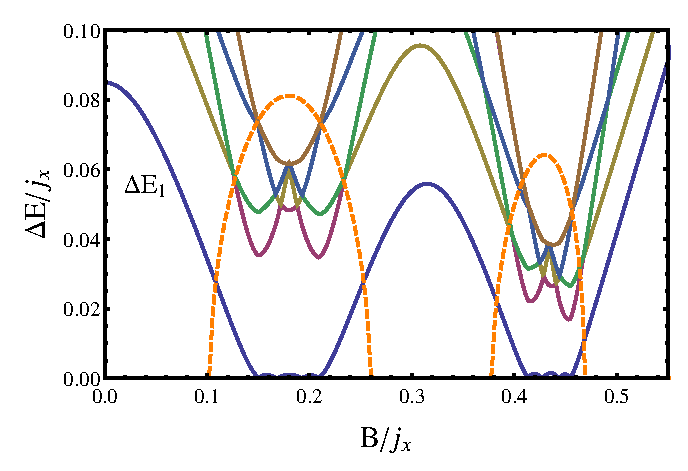
\includegraphics{fig4.ps}}}
\caption{(Color online) The lowest exact excitation energies in the $2n=8$
dimerized spin 1 chain for $\alpha=0.05$. The dashed line depicts the (scaled)
GMF parity breaking parameter $\langle S^x\rangle$. All parity transitions of
the GS are seen to take place within the  GMF parity breaking phases, where the
lowest excitation energy becomes small (and the first band 	of excitation energies
minimum).}
    \label{f4}
\end{figure}

Moreover,  the  exact  GS of the full chain exhibits $2ns$ parity transitions
as the field increases from $0$ for $\chi>0$, again reminiscent of the $2ns$
magnetization transitions of the $XX$ chain, with the last one  precisely at
the factorizing field  (\ref{Bs}). These transitions {\it are seen to be
confined within the symmetry breaking sectors of the GMF approach}, as
appreciated in Fig.\ \ref{f4} and the inset of the bottom left panel in Fig.\
\ref{f3} (they lead to small but appreciable discontinuities in all depicted
quantities for small $n$).  They indicate the crossings of the lowest negative
and positive parity exact energy levels, which lie very close in the parity
breaking sectors of  the pair MF approach, as  verified  in Fig.\ \ref{f4}.

\subsection{Higher Spins}

\subsubsection{The spin $s$ case}
The general picture remains similar for higher spins $s$  but the number of
definite parity dimerized  phases at fixed low $\alpha$ arising for $\chi>0$
and $B<B_s$ in the pair mean field becomes $2 s$, following  the $2s$ GS parity
transitions of the isolated pair for increasing fields (the last one at the
factorizing field for the pair, $B_s=J_xs \sqrt{\chi}$). Consequently, there
are three of such phases for $s=3/2$, two of each parity, as seen in Fig.\
\ref{f5} (for easier comparison between different spins, we scaled the fields
with $j_x=2J_x s$ in all Figures, such that $B_s/j_x$  and $B_c^{\rm
mf}/j_x=(1+\alpha)/2$ are spin independent, with $B_c^{\rm mf}/j_x=1$ in the
uniform ($\alpha=1$) chain). For sufficiently small  $\alpha$ the pair MF GS
can then undergo, for  $s=3/2$, up to six transitions between definite parity and
parity breaking phases (or vice versa) as $B$ increases.

 \begin{figure}
    \centerline{\scalebox{.9}{\includegraphics*{fig5.ps}}}
\caption{(Color online) Top panel: The GMF phase diagram of the spin 3/2
dimerized chain in the $\alpha$-field plane, for anisotropy
$\chi=J_y/J_x=0.75$. There are now three definite parity dimerized phases below
$B_s$ (colored sectors) if $\alpha$ is sufficiently small. Remaining details as
in Fig.\ \ref{f2}. Bottom panel: The corresponding parity breaking parameter
$\langle S^x\rangle$ for increasing fields at different fixed values of
$\alpha$ ($(0.01,0.02,0.05,0.1,05$ and $1)$. It's behavior reflects the phases
of the top panel, exhibiting  a non monotonous variation at low $\alpha$, with
``deaths and revivals'' if $\alpha\leq\alpha_c(0)$.}
    \label{f5}
 \end{figure}
 
It is also seen that the limit value of $\alpha$ for the existence of multiple
dimerized phases for $\chi>0$ decreases with  increasing spin. At zero field,
we have essentially $\alpha_c(0)\propto\Delta E/(J_x  s^2)$,  with $\Delta
E=E_1-E_0$ the energy gap to the first excited state. For $\chi=1$  ($XX$ case)
$\Delta E\propto J_x$ and hence $\alpha_c(0)\propto s^{-2}$. For $s=3/2$ we
obtain in fact $\alpha_c(0)\approx 0.06$.  However, for $\chi<1$  $\alpha_c(0)$
becomes exponentially small for large $s$, since now $\Delta E$ decreases
exponentially with increasing  spin. The behavior with $s$ of $\alpha_c(B)$ for
other fields $B<B_s$ is qualitatively similar. For $\chi=0.75$  and $s=3/2$ we
obtain $\alpha_c(0)\approx 0.019$, as seen in Fig.\ \ref{f5}.
Nevertheless, for $\alpha$ above but close to $\alpha_c(0)$ the GMF parity
breaking  parameter $\langle S^x\rangle$  continues to exhibit a non-monotonous
evolution for increasing fields, as seen for $\alpha=0.05$, where it still has
three local minima reminiscent of the dimerized phases.  On the other hand, for
$\chi<0$ there is no parity breaking if $\alpha<\alpha_c(0)$, as in the $s=1$
case.

\begin{figure}
    \centerline{\scalebox{.84}{\includegraphics*{fig6.ps}}}
\caption{(Color online) Top: Exact and GMF results for the negativity in the
dimerized spin 3/2 chain,  as a function of the (scaled) magnetic field, for
two different values of the coupling factor $\alpha$. Again $m=\langle
S_z\rangle/n$ denotes  the intensive magnetization. Bottom: The corresponding exact (solid lines) and GMF (dashed lines) results for the entanglement
entropies of a strongly coupled spin pair ($S_2$) and a single spin ($S_1$),
with the rest of the chain, as a function of the (scaled) magnetic field in the
$s=3/2$ chain for the previous values of $\alpha$.}
    \label{f6}
\end{figure}

The agreement of the GMF predictions with the exact numerical results remains
high at small values of $\alpha$, as appreciated in Fig.\ \ref{f6}. The exact
negativity $N_{12}$ and pair entanglement entropy $S_2$ exhibit, accordingly, a
non-monotonous evolution for increasing fields at low $\alpha$, with  $N_{12}$
showing for $\alpha=0.01$ $2s$ approximate plateaus at the GMF dimerized phases
separated by deep valleys at the parity-breaking sectors, before reaching the
strong field regime for $B>B_s$. On the other hand, $S_2$ is again maximum and
close to $1$ at the center of the parity breaking phases, in full agreement
with the GMF result obtained with the parity restored states (\ref{pbm}). We
also see the $2s$ approximate magnetization plateaus, as predicted by GMF.

These effects become  attenuated for $\alpha=0.05$ (right panels), where  the
fully dimerized phases for $B<B_s$ no longer exist in GMF, although  the
behavior of $N_{12}$ and $S_2$ remains non-monotonous, in agreement with
that of $\langle S^x\rangle$ in GMF. It is also seen that the GMF predictions
for the magnetization and the single spin entanglement entropy $S_1$ are very
accurate in both panels, with $s-|m|$ a good  qualitative indicator of the
latter. The exact GS of the finite chain still exhibits $2ns$ parity
transitions as $B$ increases from $0$, the last one at the factorizing field
(\ref{Bs}), although the ensuing discontinuities in the depicted quantities
become small as $s$ increases. They are again confined to the parity breaking
sectors of GMF  (i.e., to the narrow parity breaking intervals for
$\alpha=0.01$). As before, factorization at $B_s$ is reflected in the vanishing
value of $N_{12}$ at this point, while the entanglement entropies $S_1$ and
$S_2$ approach the finite limits determined by the corresponding state
(\ref{pbm}), with $S_2>S_1$ only in the vicinity of $B_s$. 	

\subsubsection{Behavior for large spin}
Let us now examine in more detail the entanglement of a single pair for
increasing spin $s$. In the top panel of Fig.\ \ref{f7} the entanglement
spectrum (the eigenvalues of the single spin reduced density matrix $\rho_1$)
is depicted as a function of the applied field for different spins. For
$\chi<1$ the reduced states become essentially rank 2 states as $s$ increases
in the whole sector $B<B_s$. The reason is that the main component of the pair
GS ($|\psi_{+}\rangle$ or $|\psi_-\rangle$) is just a parity projected rank $2$
mean field state $|\Theta_{\pm}\rangle$, i.e.,
$|\psi_\pm\rangle=\gamma|\Theta_{\pm}\rangle+|\delta\psi_{\pm}\rangle$, with
\begin{eqnarray}
|\Theta_{\pm}\rangle&=&\frac{|\theta,\theta\rangle
\pm|-\theta,-\theta\rangle}{\sqrt{2(1\pm\cos^{4s}\theta)}}=
\sqrt{p_{\pm}}|\theta_+\theta_{\pm}\rangle
+\sqrt{1-p_{\pm}}|\theta_-\theta_{\mp}\rangle  \label{statesp}\,,
\end{eqnarray}
where the last expression is its Schmidt decomposition, with
$|\theta_{\pm}\rangle=\frac{|\theta\rangle\pm|-\theta\rangle}{\sqrt{2(1\pm\cos^{2s}\theta)}}$
the local orthogonal definite parity states and $p_{-}=\frac{1}{2}$,
$p_+=\frac{(1+\cos^{2s}\theta)^2}{1-\cos^{4s}\theta}$. These states lead to a
rank $2$ $\rho_1$ with eigenvalues $(p_{\pm},1-p_{\pm})$. By optimizing the
angle $\theta$ it is found that the overlap
$|\gamma|=|\langle\Theta_{\pm}|\psi_{\pm}\rangle|$ exceeds 0.9 for all field
and spin values, with  $|\langle\Theta_{\pm}|\psi_{\pm}\rangle|\agt 0.95$ for
all fields if $s\geq 5$. The states (\ref{statesp}) become of course the {\it
exact} pair GS at the factorizing field $B_s$, with the overlap staying above
0.99 for $B>B_s$. We can verify from Fig.\ \ref{f7} that the contribution of
$|\delta\psi_{\pm}\rangle$ to the entanglement spectrum is negligible.

\begin{figure}
    \centerline{\scalebox{.9}{\includegraphics{fig7.ps}}}
\caption{(Color online) Top: The entanglement spectrum of the GS of a spin $s$
pair as a function of the applied field for $s=5$ and $\chi=J_y/J_x=0.75$
(left) and $1$ (right). In the anisotropic case  it is formed essentially by
just two degenerate eigenvalues below the factorizing field (as described by
Eq.\ (\ref{statesp})), whereas in the $XX$ case (right) there are several
non-vanishing eigenvalues (two-fold degenerate), in agreement with the gaussian
profile (\ref{g}) (shown in the bottom right panel for $s=5$ and $20$, together with the exact results, indistinguishable from (\ref{g})).  
Bottom: The negativity of the pair as a function of the
(scaled) magnetic field for different spin values and $\chi=0.75$ (left), where
$s=1/2,1,\frac{3}{2},2,5,10$ and $\infty$ (bosonic limit, Eq.\ (\ref{N12b})),
and $\chi=1$ (right), where $s=1/2,1,\frac{3}{2},2,5,10,20$ and $50$. Notice
the different scales.}
    \label{f7}
\end{figure}

Nonetheless, its contribution to the negativity is important if $\chi$ is not
too small. For $|B|<B_s$ the states $|\Theta_{\pm}\rangle$ lead essentially to
an almost constant negativity  $N_{\pm}\approx 1/2$ for large $s$ if $\theta$
is not too small, i.e.,
$N(|\Theta_{+}\rangle)=\frac{1-\cos^{4s}\theta}{2(1+\cos^{4s}\theta)}$,
$N(|\Theta_-\rangle)=\frac{1}{2}$, which for $B<B_s$ lies below the exact
value. The latter remains, however, {\it  bounded as the spin $s$ increases} if
$|\chi|<1$. Its  maximum at zero field is in fact attained at low finite spin
($s\approx 2$ for $\chi=0.75$, as seen in the bottom left panel of Fig.\
\ref{f7}).

For large $s$ and $\chi<1$, the correction $|\delta\psi_{\pm}\rangle$ and its
effect on the pair negativity and entanglement entropy can be determined
through a bosonic RPA approach \cite{MRC.10}. Around the normal mean field
phase ($B>B_c=J_xs$) such approach implies at lowest order the replacements
$S_i^z\approx b^\dagger_i b_i-s$, $S_i^{+}\approx b^\dagger_{i}$, $S_i^-\approx
b_i$ with $b_i$, $b^\dagger_i$ bosonic operators
($[b_i,b^\dagger_j]=\delta_{ij}$), while around the parity-breaking mean field
a similar replacement is to be applied to the rotated spin operators
$S_i^{z'}$, $S_{i}^{\pm'}$, with $S_i^{-'}|\Theta\rangle=0$. Taking into
account parity restoration effects, such bosonisation leads to the analytic
expression
\begin{equation} N_{12}=\left\{\begin{array}{lr}f+\sqrt{f(f+1)}\,,&\;|B|>B_c=J_x s\\
2[f+\sqrt{f(f+1)}]+1/2\,,&\;|B|<B_c\end{array}\right.\label{N12b}\end{equation}
where $f$ is the  average single site bosonic occupation number,
\begin{equation}f={\textstyle\frac{1}{2}(\sqrt{1+\frac{\lambda^2 -\omega_m^2}{\omega_+\omega_-}}-1)}
\,,\end{equation}
with $\lambda=|B|\;(B_c)$ for $|B|>B_c\;(<B_c)$, $\omega_m=\frac{\omega_{+}+\omega_-}{2}$
and $\omega_{\pm}$ the bosonic eigenfrequencies
\begin{equation} \omega_{\pm}=\left\{\begin{array}{lr}
B_c\sqrt{(1\pm(B/B_c)^2)(1 \pm \chi)}\,,&\;|B|<B_c
\\B_c\sqrt{(B/B_c\pm 1)(B/B_c\pm \chi)}\,,&\;|B|>B_c\end{array}\right.\,.\end{equation}
The exact results for the negativity are verified  to approach the previous
finite and $s$-independent bosonic limit for large spin in the anisotropic case
$\chi<1$ (bottom left panel in Fig.\ \ref{f7}). The corresponding pair
entanglement entropy is given by $S_2=-f\log_2 f+(f+1)\log_2(f+1)+\delta$,
where $\delta=0$ ($1$) for $B>B_c$ ($<B_c$) \cite{MRC.10}.

However, in the $XX$ case $\chi=1$ ($J_y=J_x$)  the behavior for high spin is
different. Here $H_{12}$ commutes with the total spin component
$S^z_t=S_1^z+S_2^z$, implying that the parity breaking solution of the pair
mean field is actually breaking a continuous symmetry. Symmetry restoration
implies then integration over all rotations around the $z$ axis (i.e.,
projection onto definite magnetization) and the previous approach (Eqs.\
(\ref{statesp})--(\ref{N12b})) no longer holds. Nevertheless, since the exact
GS has now definite magnetization $M$, it is of the form
\begin{equation}
|\psi_M\rangle=\sum_{m=-s}^{M+s}\alpha_M^m|m,M-m\rangle\,,\;\;\;(\chi=1)\label{sm}
\end{equation}
for $M\leq 0$, with $M$ determined by the applied transverse field ($M\approx -2s [B/B_c]$ for
$B\leq B_c$, $[\ldots]$ integer part) and all $\alpha_M^m$ of the same sign for
$J_x>0$ in (\ref{H1}). Eq.\ (\ref{sm}) is directly its Schmidt decomposition,
implying that the single spin reduced state will have eigenvalues
$|\alpha_M^m|^2$, two-fold degenerate for $m\neq M/2$
($\alpha_M^m=\alpha_M^{M-m}$), leading to the entanglement spectrum of the top
right panel in  Fig.\ \ref{f7}. The number  of non-zero eigenvalues (the
Schmidt rank of $|\psi_M\rangle$) will then be  $2s+1-|M|$. For $|M|$ not too close to $2s$ the coefficients will have essentially a {\it gaussian distribution}, 
as appreciated in the bottom right panel of Fig.\ \ref{f7},  
\begin{equation}\alpha_M^m\propto e^{-(m-M/2)^2/(4\sigma_M^2)}\,,\;\;\;\sigma_M\approx r_M s\label{g}\end{equation}
where for $s$ not too small, the fluctuation $\sigma_M^2\approx
\langle(S^z_1-M/2)^2\rangle$ will be {\it proportional
to the spin $s$}, as obtained from the high spin expansion of the exact eigenvector equation. The factor $r_M$ decreases for increasing $|M|$ and for $M=0$ it is given 
by $r_0=1/(2\sqrt{2})\approx 0.35$, whereas for $|M|=s/2$,   
$r_{s/2}\approx 0.32$. The overlap between the gaussian expression
and exact distribution exceeds $0.999$ for $s\geq 5$ at $M=0$. 

Let us remark  that for two spins $s$ coupled to total spin $2s$ and magnetization $M$, the corresponding distribution of the  $\alpha_M$'s are  Clebsch-Gordan coefficients, which  also lead to a gaussian distribution for high $s$ and $|M|$ not close to $2s$, with a width also proportional to $s$ but slightly smaller (at zero field, $\sigma_0^2\approx s/4<s/(2\sqrt{2}))$. Hence, the actual distribution in the GS of the $XX$ pair contains small admixtures from lower values of the total spin, as $H_{12}$ does not commute with it.  

\begin{figure}
\centerline{\scalebox{1.}{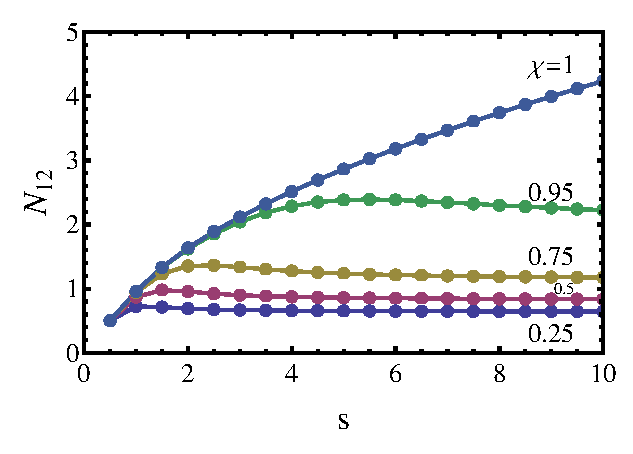
\includegraphics{fig8.ps}}} \caption{(Color online)
Negativity of a pair for increasing spin $s$ at zero field for different
anisotropies $\chi=J_y/J_x$. For $\chi<1$ they saturate, approaching the limit values (\ref{N12b}), while for $\chi=1$ they increase as $\sqrt{s}$, as given by Eq.\ (\ref{N12a}) 
(indistinguishable from the exact result for $s\geq 1$ on this scale).}
   \label{f8}
\end{figure}

Therefore, the negativity of the pair can be estimated through the gaussian
approximation, which leads, using Eq.\ (\ref{N12p}), to
\begin{equation}N_{12}\approx \sqrt{2\pi\sigma_M^2}-{\textstyle\frac{1}{2}}\approx
 \sqrt{2\pi r_M s}-{\textstyle\frac{1}{2}}\,.\label{N12a}\end{equation}
Consequently, the entanglement is {\it unbounded} for increasing spin,  with
$N_{12}$  increasing as $\sqrt{s}$ for $\chi=1$, as verified in the bottom
right panel of Fig.\ \ref{f7} and in Fig.\ \ref{f8}.  The  entanglement entropy
of the pair becomes, similarly,  $S(\rho_1)\approx \frac{1}{2\ln 2}[1+\ln(2\pi
\sigma_M^2)]\approx \frac{1}{2\ln 2}[1+\ln(2\pi r_M s)]$.

The previous behavior of the pair entanglement with $s$ holds also for  an
$XXZ$ coupling $-J(S_1^xS_2^x+S_1^yS_2^y)-J_zS_1^zS_2^z$ if  $J_z>-J$ ($J>0$),
in which case the coefficients $\alpha_M^m$ remain gaussian with finite width
$\sigma_M$.  However, in the  AFM case $J_z=-J$, $J>0$ (equivalent through
local rotations to $J_z=J<0$) at zero magnetization, the gaussian becomes
uniform and the pair GS becomes {\it maximally entangled}, i.e.
$|\alpha_m^0|=1/\sqrt{2s+1}$ $\forall$ $m$ (with $|\psi_0\rangle$ becoming the
singlet state with zero total angular momentum for $J_z=J<0$). Such state leads
then to $N_{12}=s$ and $S(\rho_1)=\log_2(2s+1)$, with maximum fluctuation
$\langle {S_1^z}^2\rangle=s(s+1)/3$.


\section{Conclusions\label{IV}}
We have analyzed the behavior of pair entanglement and magnetization in
dimerized spin-$s$ chains with $XY$ couplings in a transverse field. It was
shown that for weak coupling between pairs, these quantities can be correctly
described by a self-consistent pair mean field approach, which can predict up
to $2s$ dimerized phases below the factorizing field if $\alpha$ is
sufficiently low and $\chi>0$, lying between $S_z$ parity breaking phases. The
dimerized sectors are visible through the concomitant approximate plateaus in
the chain magnetization and pair negativity $N_{12}$ and the low values of the
pair entanglement $S_2$ with the rest of the chain, while the intermediate
parity breaking phases through the minima in $N_{12}$ and maxima in $S_2$,
together with  the linear increase in the magnetization. These effects can be
all  described by the pair mean field approach if basic parity restoration is
employed in parity breaking phases. Magnetization was also seen to correlate
with the entanglement entropy $S_1$ of a single spin, which is larger than
$S_2$ except in the vicinity of $B<B_s$,  indicating dimerization. These multiple phases arise below
increasingly lower values of the coupling between pairs as $s$ increases, with
the $XX$ case being more favorable. Non-monotonous magnetic behavior  of
$N_{12}$ and $S_2$ nevertheless subsists for higher couplings, in agreement
with the non-monotonicity of the parity breaking parameter of the pair mean
field.

It was also shown that the isolated pair negativity rapidly saturates as $s$
increases in the anisotropic $XY$ case, in agreement with the predictions of a
mean field plus RPA treatment with parity restoration, whereas in the $XX$ case
it increases as $s^{1/2}$, following a gaussian description, being then
intermediate between the $XY$ and the full AFM case.

These results show that interesting phases with non-trivial entanglement and
magnetic properties can arise for non-homogeneous couplings, leading to regimes still far from the  bosonic-like large $s$ limit.
Generalized self consistent mean field treatments based on non-trivial units
like pairs or clusters can provide a good description of such systems in these
regimes, specially if supplemented with symmetry restoration, offering a
convenient starting point for more complex treatments.

The authors acknowledge support from CONICET (AB, NC, JMM), and CIC
(RR) of Argentina.

\begin{thebibliography}{999}
\bibitem{Am.08} L.\ Amico, R.\  Fazio, A.\ Osterloh, V.\ Vedral, Rev.\ Mod.\ Phys.\ {\bf 80}, 517 (2008).
\bibitem{ECP.10}J.\ Eisert, M.\ Cramer, M.B.\ Plenio, Rev.\ Mod.\ Phys.\ {\bf 82}, 277 (2010).
\bibitem{ON.02} T. J. Osborne, M.A.\ Nielsen, Phys.\ Rev.\ A {\bf 66}, 032110 (2002). 
\bibitem{VLRK.03}G.\ Vidal, J.I.\ Latorre, E.\ Rico, A.\ Kitaev, Phys.\ Rev.\ Lett.\ {\bf 90}, 227902 (2003).
\bibitem{NC.00} M.A.\ Nielsen, I.L.\ Chuang, {\em Quantum Computation and Quantum Information}
(Cambridge Univ. Press, Cambridge, UK, 2000).
\bibitem{HR.06} S.\ Haroche, J.M. Raimond {\em Exploring the Quantum}
		(Oxford,  Univ. Press, Oxford, UK (2006).	
\bibitem{PC.04} D.\ Porras, J.I.\ Cirac, Phys.\ Rev.\ Lett.\ {\bf 92}, 207901 (2004).
\bibitem{GA.14} I.M.\ Georgescu, S.\ Ashhab, and F.\ Nori, Rev.\ Mod.\ Phys. {\bf 86}, 153 (2014). 
	\bibitem{BR.12} R. Blatt and C.F.\ Roos, Nat.\ Phys. \ {\bf 8}, 277 (2012).
	\bibitem{SR.15} C.\ Senko, P.\ Richerme, J.\ Smith, A.\ Lee, I.\ Cohen, A.\ Retzker, C.\ Monroe, 
	Phys.\ Rev.\  X {\bf 5}, 021026 (2015).
	\bibitem{B.16} R.\ Barends et al  Nature {\bf 534} 222 (2016);
	R.\ Barends et al Phys.\ Rev.\ Lett.\ {\bf 111}, 080502 (2013).
	\bibitem{LS.12} M.\ Lewenstein, A.\ Sanpera, V.\ Ahufinger, {\it Ultracold Atoms
		in Optical Lattices}, Oxford Univ.\ Press, UK, 2012.
\bibitem{Pr.75} J.H.H.\ Perk, H.W.\ Capel, M.J.\ Zuilhof, Th.J.\ Siskens,
Phys.\ A {\bf 81}, 319 (1975);
Th.J.\ Siskens, H.W.\ Capel, J.H.H.\ Perk, Phys.\ Lett.\ A {\bf 53}, 21 (1975).
\bibitem{Pr.77} J.H.H.\ Perk,  H.W.\ Capel, Th.J.\ Siskens, Phys.\ A {\bf 89}, 304 (1977);
J.H.H.\ Perk, H.W.\ Capel, Phys.\ A {\bf 92}, 163 (1978);
 J.H.H.\ Perk, H.\ Au-Yang, J.\ Stat.\ Phys.\ {\bf 135}, 599 (2009).
\bibitem{FM.07} E.I.\ Kutznetsova, E.B.\ Fel'dman, JETP.\ Lett.\ {\bf 102}, 882 (2006);
E.B.\ Fel'dman, M.G.\ Rudavets, JETP.\ Lett.\ {\bf 81}, 47 (2005).
S.I.\ Doronin, A.N.\ Pyrkov, E.B.\ Fel'dman,, JETP Lett.\ 85, 519 (2007).
\bibitem{MG.69} C.K.\ Majundar, D.K.\ Gosh, J.\ Math.\ Phys.\ {\bf 10}, 1388 (1969);
{\it ibid} {\bf 10}, 1399 (1969); B.S.\ Shastry and B.\ Sutherland,
Phys.\ Rev.\ Lett.\ {\bf 47}, 964  (1981).
\bibitem{S.05}H.J.\ Schmidt, J.\ Phys.\ A {\bf 38} 2123 (2005).
\bibitem{KSV.07} D.\ Kaszlikowski, W.\ Son, V.\ Vedral, Phys.\ Rev.\ A {\bf 76}, 054302
(2007).
\bibitem{HXG.08} M.-G.\ Hu, K.\ Xue, M.-L.\ Ge, Phys.\ Rev.\ A {\bf 78}, 052324
(2008).
\bibitem{HH.11} J.\ Sirker, A.\  Herzog, A.M.\ Oles, P.\ Horsch, Phys.\ Rev.\ Lett. {\bf 101} 157204 (2008);
A.\ Herzog, P.\ Horsch, A.M.\ Oles, J.\ Sirker, Phys.\ Rev.\ B {\bf 84} 134428 (2011).
\bibitem{Mn.14} P.\ Merchant, B.\ Normand, K.W.\ Kramer, M.\ Boehm, D.F.\ McMorrow, Ch.\ R�egg, 
Nature Phys.\ {\bf 10}, 373 (2014).
\bibitem{GG.09}G.L.\ Giorgi, Phys.\ Rev.\ B {\bf 79}, 060405(R) (2009); {\bf 80},
019901(E)(2009).
\bibitem{CRM.10} N.\ Canosa, R.\ Rossignoli, J.M.\ Matera, Phys.\ Rev.\ B {\bf 81},
054415 (2010).
\bibitem{BRCM.15} A.\ Boette, R.\ Rossignoli, N.\ Canosa, J.M.\ Matera, 
Phys.\  Rev.\ B {\bf 91}, 064428 (2015). 
\bibitem{LM.15} C.A.\ Lamas, J.M.\ Matera,  Phys.\ Rev.\ B{\bf 92}, 115111 (2015);
J.M.\ Matera,  C.A.\ Lamas,  J.\ Phys.:\ Condens.\ Matter {\bf 26} 326004 (2014).
\bibitem{ORSB.15}V.\ Ohanyan, O.\ Rojas, J.\ Stre\v cka, S.\ Bellucci, 
Phys.\ Rev.\ B {\bf 92}, 214423 (2015). 
\bibitem{ZZ.14}  T.\ Ramos, H.\ Pichler, A.J.\ Daley, P.\ Zoller, 
Phys.\ Rev.\ Lett.\ {\bf 113}, 237203 (2014). 
A.W.\ Glaetzle, M.\ Damonte, R.\ Nath, C.\ Gross, I.\ Bloch, P.\ Zoller, 
Phys.\ Rev.\ Lett.\ {\bf 114} 173002 (2015); I.\ Bloch, J.\ Dalibard, 
W.\ Zwerger, Rev.\ Mod.\ Phys.\ {\bf 80}, 885 (2006).
\bibitem{LSM.61} E.\ Lieb, T.\  Schultz, D.\ Mattis, Ann.\ Phys.\ {\bf 16}
407 (1961).
\bibitem{MRC.10}J.M.\ Matera, R.\ Rossignoli, N.\ Canosa, Phys.\ Rev.\ A {\bf 82}, 052332 (2010).
\bibitem{KTM.82} J.\ Kurmann, H.\ Thomas, G.\ M\"uller, Phys.\ {\bf A} 112, 235 (1982).
\bibitem{VW.02} G.\ Vidal and R.F.\ Werner, Phys.\ Rev.\ A {\bf 65}, 032314 (2002).
\bibitem{ZHSL.99}K.\ Zyczkowski, P.\ Horodecki, A.\ Sanpera, M.\ Lewenstein,
Phys.\ Rev.\ A {\bf 58}, 883 (1998); K.\ Zyczkowski, {\it ibid.} {\bf 60}, 3496 (1999).
\bibitem{RCM.08}  R.\ Rossignoli,
N.\ Canosa, J.M.\ Matera, Phys.\  Rev.\ A {\bf 77}, 052322
(2008).
\bibitem{RCM.09} R.\ Rossignoli,  N.\ Canosa, J.M.\ Matera, Phys.\  Rev.\ A {\bf 80}, 062325
(2009).
\bibitem{W.89}R.F.\ Werner, Phys.\ R	ev.\ A {\bf 40}, 4277 (1989).
\bibitem{SR.09} S.\ Rachel, Euro.\ Phys.\ Lett.\ {\bf 86}, 37005 (2009).
\bibitem{MV.12}F.\ Michaud, F.\ Vernay, S.R.\ Manmana, and F.\ Mila, Phys.\ Rev.\ Lett.\ {\bf 108}, 127202 (2012); M.\ Lajko, P.\ Sindzingre, and K.\ Penc, ibid.\ {\bf 108}, 017205 (2012).
\bibitem{KM.08}V.\ Karimipour and L.\ Memarzadeh, Phys.\ Rev.\ {\bf B 77}, 094416 (2008):
\end{thebibliography}
\end{document}


